\documentclass[tikz,border=6pt]{standalone}
\usepackage{pgfplots}
\usepackage{amsmath}
\usetikzlibrary{
  arrows.meta,
  backgrounds,
  calc,
  fit,
  matrix,
  positioning,
  shapes.callouts,
  shapes.geometric,
  shapes.misc
}
\pgfplotsset{compat=1.18}

\definecolor{archInk}{HTML}{1F2933}
\definecolor{archBlue}{HTML}{0B4F6C}
\definecolor{archTeal}{HTML}{1B998B}
\definecolor{archGold}{HTML}{D98E04}
\definecolor{archRose}{HTML}{C44536}
\definecolor{archSage}{HTML}{7A9E7E}
\definecolor{archMist}{HTML}{E9F1F7}
\definecolor{archSand}{HTML}{F4F1DE}
\definecolor{archSlate}{HTML}{5C677D}
\definecolor{archStone}{HTML}{C8D0D9}

\tikzset{
  every node/.style={font=\sffamily\small, text=archInk},
  axis label/.style={font=\sffamily\footnotesize, text=archInk},
  panel/.style={
    rounded corners=6pt,
    draw=archSlate,
    line width=0.9pt,
    fill=white
  },
  stage/.style={
    panel,
    fill=archMist,
    minimum height=1.5cm,
    inner sep=7pt,
    align=left
  },
  note/.style={
    panel,
    fill=archSand,
    inner sep=7pt,
    align=left
  },
  verdict/.style={
    panel,
    fill=archTeal!12,
    inner sep=7pt,
    align=left
  },
  kill/.style={
    panel,
    fill=archRose!12,
    draw=archRose,
    inner sep=7pt,
    align=left
  },
  muted/.style={
    panel,
    fill=archStone!20,
    draw=archStone!80!archInk,
    inner sep=6pt,
    align=left
  },
  link/.style={
    -{Latex[length=3mm,width=1.7mm]},
    line width=1.0pt,
    draw=archBlue
  },
  dashedlink/.style={
    -{Latex[length=3mm,width=1.7mm]},
    line width=1.0pt,
    draw=archRose,
    dashed
  }
}

\pgfplotsset{
  every axis/.append style={
    line width=0.9pt,
    tick style={draw=archSlate},
    axis line style={draw=archSlate},
    label style={font=\sffamily\small, text=archInk},
    ticklabel style={font=\sffamily\footnotesize, text=archInk},
    legend style={
      draw=none,
      fill=white,
      font=\sffamily\footnotesize,
      text=archInk
    },
    title style={font=\sffamily\small\bfseries, text=archInk},
    grid style={draw=archStone},
    major grid style={draw=archStone},
    minor grid style={draw=archStone!70}
  }
}

\begin{document}
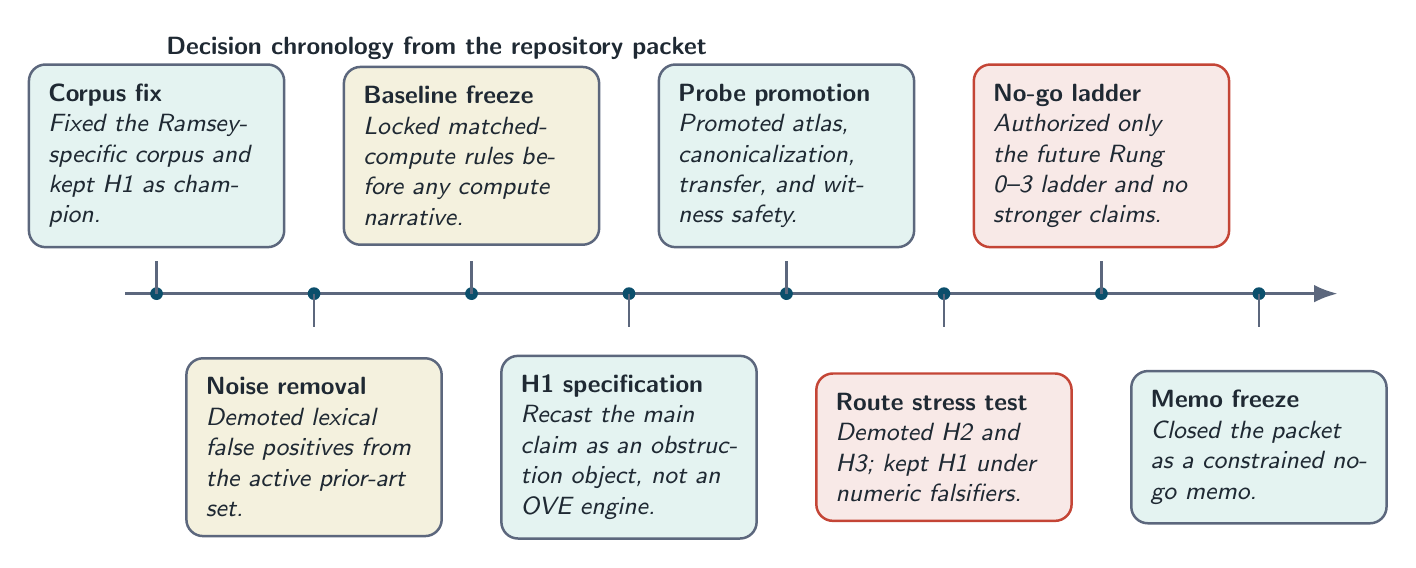
\begin{tikzpicture}[x=2cm,y=1cm]
  \draw[archSlate, line width=1.1pt, -{Latex[length=3mm]}] (-0.2,0) -- (7.5,0);

  \foreach \x/\title/\text/\style/\y in {
    0/{Corpus fix}/{Fixed the Ramsey-specific corpus and kept H1 as champion.}/verdict/1.75,
    1/{Noise removal}/{Demoted lexical false positives from the active prior-art set.}/note/-1.95,
    2/{Baseline freeze}/{Locked matched-compute rules before any compute narrative.}/note/1.75,
    3/{H1 specification}/{Recast the main claim as an obstruction object, not an OVE engine.}/verdict/-1.95,
    4/{Probe promotion}/{Promoted atlas, canonicalization, transfer, and witness safety.}/verdict/1.75,
    5/{Route stress test}/{Demoted H2 and H3; kept H1 under numeric falsifiers.}/kill/-1.95,
    6/{No-go ladder}/{Authorized only the future Rung 0--3 ladder and no stronger claims.}/kill/1.75,
    7/{Memo freeze}/{Closed the packet as a constrained no-go memo.}/verdict/-1.95
  }{
    \fill[archBlue] (\x,0) circle (2.3pt);
    \draw[archSlate, line width=0.9pt] (\x,0) -- (\x,{0.42*sign(\y)});
    \node[\style, text width=2.75cm, anchor=center] at (\x,\y) {
      \textbf{\title}\\
      \textit{\text}
    };
  }

  \node[font=\sffamily\bfseries\small, text=archInk, anchor=west] at (0,3.12)
    {Decision chronology from the repository packet};
\end{tikzpicture}
\end{document}
